% !TEX root = ../main.tex
\section{Association Elements} \label{sec:associationelements}
	Going through the alphabet I was able to find 13 patterns that matched a letter from the alphabet. Out of the 13 letters it was 9 that had a sigificant number of apperences in the sample data. 

  By iterating throuh a list og sequences formin a patter I was able to find 385 patterns in the dataset matching one of the 13 letters. Compared to the total number of patterns (3393) it is 11,4\% of the patterns in the collected data are forming a letter.

  \clearpage

    \begin{figure}[H]
      \centering
      \vspace{1.5cm}

      \subfigure[The letter C]{
        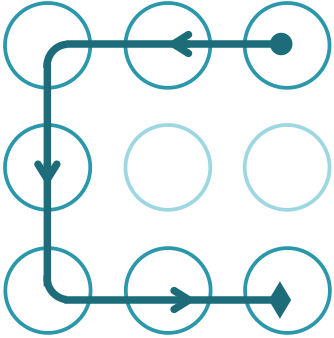
\includegraphics[width=0.27\textwidth]{pics/letters/bokstavenC.png}\hspace{0.6cm}
      }
      \subfigure[The letter L (big)]{
        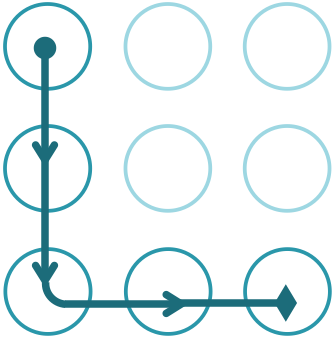
\includegraphics[width=0.27\textwidth]{pics/letters/bokstavenL.png}\hspace{0.6cm}
      }
      \subfigure[The letter L (small)]{
        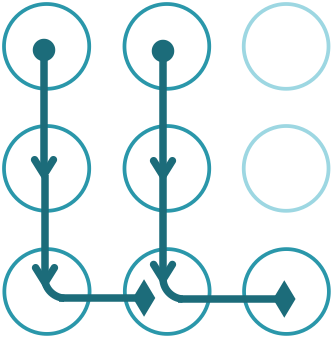
\includegraphics[width=0.27\textwidth]{pics/letters/bokstavenLitenL.png}
      }

      \vspace{0.5cm}

      \subfigure[The letter M]{
        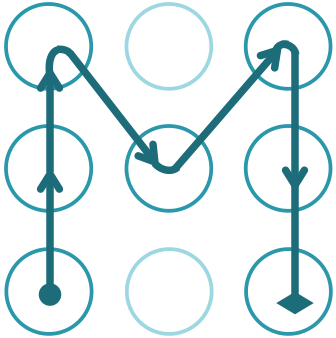
\includegraphics[width=0.27\textwidth]{pics/letters/bokstavenM.png}\hspace{0.6cm}
      }
      \subfigure[The letter N]{
        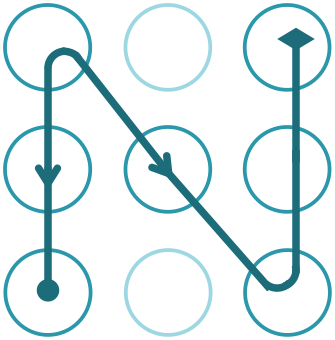
\includegraphics[width=0.27\textwidth]{pics/letters/bokstavenN.png}\hspace{0.6cm}
      }
      \subfigure[The letter O]{
        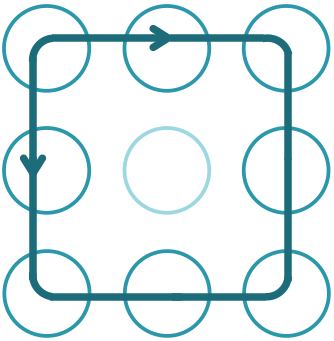
\includegraphics[width=0.27\textwidth]{pics/letters/bokstavenO.png}
      }

      \vspace{0.5cm}

      \subfigure[The letter S]{
        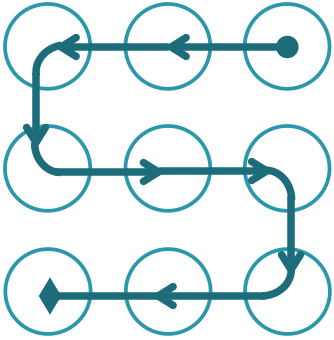
\includegraphics[width=0.27\textwidth]{pics/letters/bokstavenS.png}\hspace{0.6cm}
      }
      \subfigure[The letter U]{
        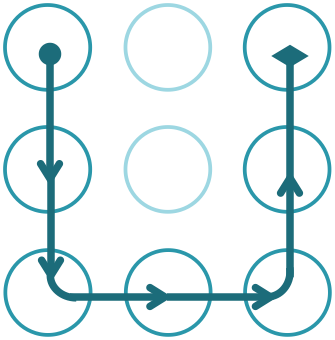
\includegraphics[width=0.27\textwidth]{pics/letters/bokstavenU.png}\hspace{0.6cm}
      }
      \subfigure[The letter Z]{
        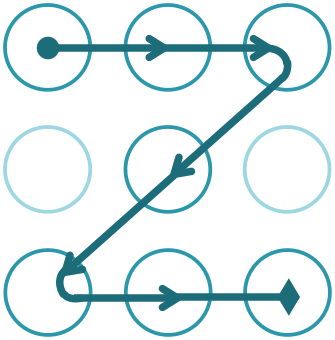
\includegraphics[width=0.27\textwidth]{pics/letters/bokstavenZ.png}
      }

      \vspace{0.5cm}
      \caption{Most frequent patterns forming letters from the alphabet}
    \end{figure}

  \clearpage